\chapter{Introduction}
\label{ch:introduction}
Speed of change\\
Only constant is change\\

\acrfull{vuca}\\
The challenge\\

In this thesis, the researcher defines how and with which \acrfull{ea} concepts \acrshort{ea} can be used to steer an \acrfull{isv} towards being \gls{antifragile} in the Public Sector Market.

\section{Context}
\label{sec:context}
The researcher is working as a Chief Architect for an \acrshort{isv} specialised in delivering software and services to the local governments in The Netherlands, such as the municipalities, the provinces, and the regional water authorities. The local governments embraced the digital transformation, and because of this the pace of change is increasing rapidly \needsref. 

\section{Structure of the thesis}
\label{sec:structure}
In chapter \ref{ch:introduction} the context of the research is set, the core concepts of \acrshort{ea} and \glspl{antifragile} are introduced together with the contextual concepts of \acrshort{isv} and the Public Sector Market. In chapter \ref{ch:theoreticalbackground} the theoretical background is given on the research. Chapter \ref{ch:research-methodology} explains the used methodology for the research.

\section{Introduction of the Public Sector Market}
\label{sec:intropublicsector}

\section{Introduction of Indepenent Software Vendor}
\label{sec:introisv}

\section{Introduction of the concept Enteprise Architecture}
\label{introea}
\acrfull{ea} is a discipline for proactively and holistically leading enterprise responses to disruptive forces by identifying and analysing the execution of change toward desired business vision and outcomes. \acrshort{ea} delivers value by presenting business and IT leaders with signature-ready recommendations for adjusting policies and projects to achieve targeted business outcomes that capitalise on relevant business disruptions \parencite{Gartner}.\par
\textcite{White2018} states that the organisation’s business requirements guide \acrshort{ea} — it helps layout how information, business and technology flow together. \acrshort{ea} has become a priority for businesses trying to keep up with new technologies such as the cloud, \acrfull{iot}, machine learning and other emerging trends that will prompt digital transformation.

\section{Introduction of the concept of Antifragility}
\label{sec:introantifragility}
\textcite{Taleb2008} describes a black swan as an event that 1) is so rare that even the possibility that it might occur is unknown, 2) has a catastrophic impact when it does occur, and 3) is explained in hindsight as if it were actually predictable. For extremely rare events, \citeauthor{Taleb2008} argues that the standard tools of probability and prediction, such as the normal distribution, do not apply since they depend on large population and past sample sizes that are never available for rare events by definition. Extrapolating, using statistics based on observations of past events is not helpful for predicting black swans, and might even make us more vulnerable to them. In his book \Gls{antifragile}, \textcite{Taleb2013} states that the way to survive a black swan event is to be \gls{antifragile}.\par
Most people answer that the opposite of \gls{fragile} is \gls{robust}, \gls{resilient}, solid, or something of the sort. However, the \gls{resilient}, \gls{robust} (and company) are items that neither break nor improve, so you would not need to write anything on them — have you ever seen a package with \gls{robust} in thick green letters stamped on it? Logically, the exact opposite of a \gls{fragile} parcel would be a package on which one has written, please mishandle or please handle carelessly. Its contents would not just be unbreakable but would benefit from shocks and a wide array of trauma \parencite{Taleb2013}.

\section{Problem statement}
\label{sec:problemstatement}

\section{Research questions}
\label{sec:research-questions}

\subsection{Main research question}
\label{sub:main-research-question}
\acrshort{ea} facilitates an organisation in assessing the impact of change and making recommendations for target states that support business objectives. \acrshort{ea} guides an organisation in changing. \acrshort{ea} can help organisations in changing into a state of \gls{antifragility}. However, what are the success factors of enterprise architecture to accomplish \gls{antifragility}?
\begin{figure}[!h]
	\centering
	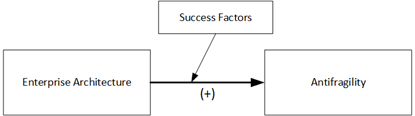
\includegraphics[width=0.7\linewidth]{images/conceptmodel}
	\caption[Research Model]{Research Model}
	\label{fig:researchmodel}
\end{figure}
\begin{center}
\framebox{
\begin{minipage}{0.9\linewidth}
What are, for an \acrlong{isv}, the success factors of \acrlong{ea} for \gls{antifragility} in the public sector market?
\end{minipage}
}
\end{center}

\subsection{Sub-questions}
\label{sub:sub-questions}

\begin{enumerate}
	\item{Sub-question 1}
	\item{Sub-question 2}
\end{enumerate}
